\chapter{Convenzioni e Notazioni}
\label{Notazioni}
%
\subsection{Sistemi di Riferimento}
La convenzione utilizzata per definire gli assi del sistema di riferimento della vettura è la \ac{ISO} 8855.

\begin{figure}[h!]
	\centering
	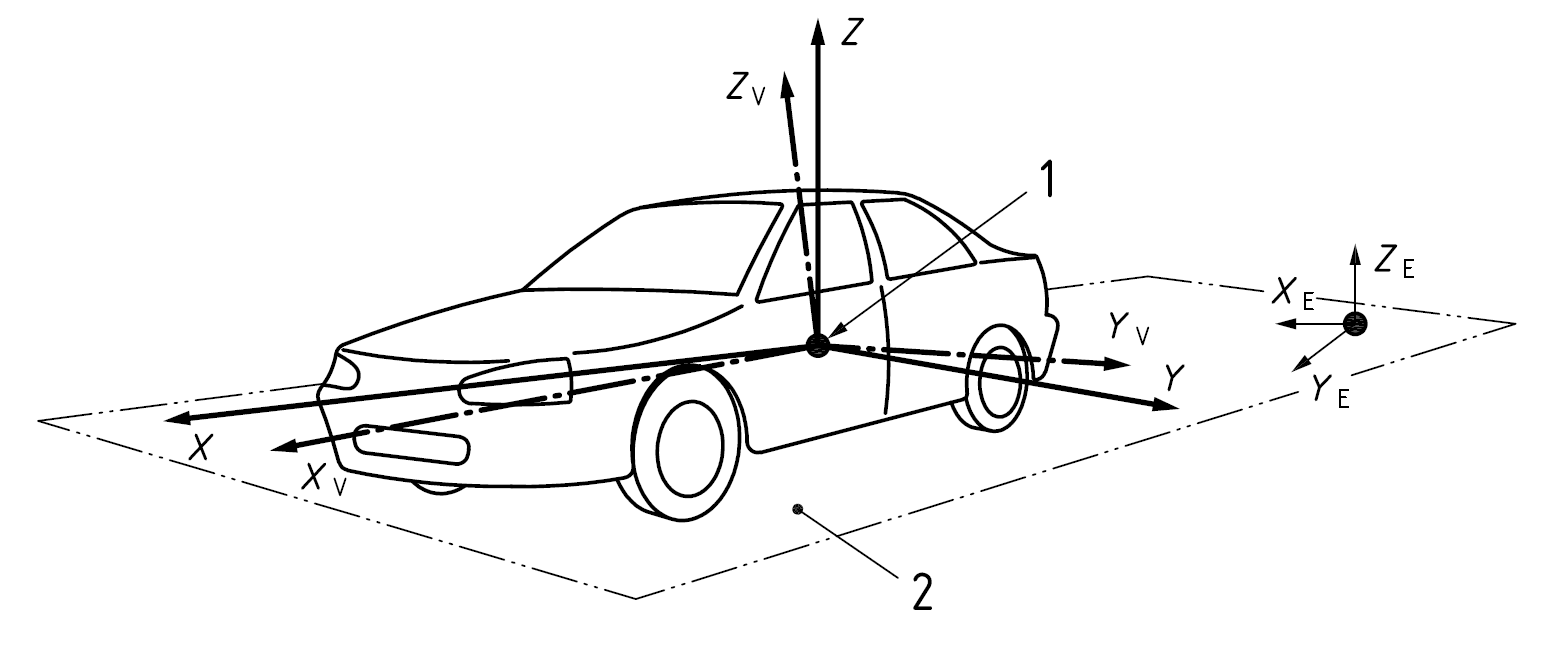
\includegraphics[width=0.8\linewidth]{Figures/iso_convention}
	\caption{Rappresentazione degli assi del sistema di riferimento della vettura secondo la convenzione ISO-V.}
	Da: \citeauthor{Ginebra}, \citetitle{Ginebra}.
	\label{isoconventionv}
\end{figure}

\noindent
Il sistema di riferimento della ruota è conforme alla convenzione \ac{ISO}-V, la cui disposizione degli assi è illustrata nella \figurename{ \ref{isoconventionc}}. L'origine del sistema di riferimento del vettore ruota è posta in corrispondenza del centro della ruota mentre posizione e orientamento relativi rispetto al sistema di riferimento del telaio sono definiti attraverso il modello della sospensione descritto in \cite{Larcher}.

\begin{figure}[h!]
	\centering
	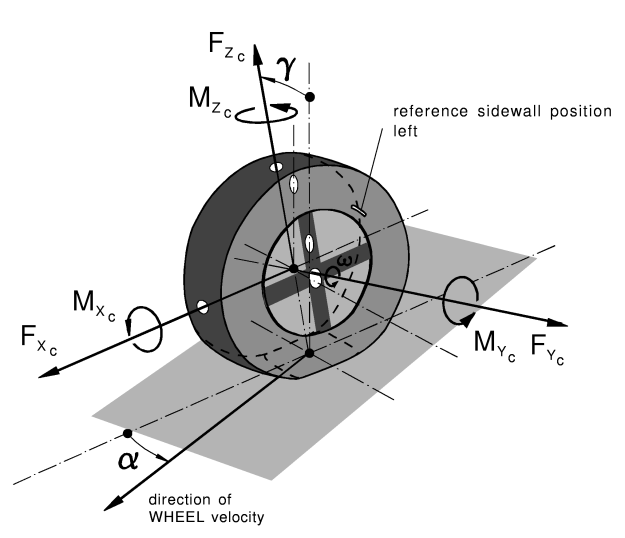
\includegraphics[width=0.6\linewidth]{Figures/iso_convention_wheel}
	\caption{Rappresentazione degli assi  del sistema di riferimento dello pneumatico secondo la convenzione ISO-C.}
	Da: Documentazione \texttt{MFeval}.
	\label{isoconventionc}
\end{figure}
%
\subsection{Matrice di Trasformazione}
Per descrivere sia l'orientamento che la posizione di un sistema di assi nello spazio, viene introdotta la matrice roto-traslazione, chiamata anche matrice di trasformazione. Questa notazione permette di impiegare le operazioni matrice-vettore per l'analisi di posizione, velocità e accelerazione. La forma generale di una matrice di trasformazione è del tipo:
%
\begin{equation}
T_m = \left[
\begin{array}{ccc|c}
& & & O_{mx}\\
\multicolumn{3}{c|}{\multirow{3}{*}{\raisebox{20mm}{\scalebox{1.5}{$[R_m]$}}}} & O_{my}\\
& & & O_{mz}\\ \hline
0 & 0 & 0 & 1
\end{array}\right]
\end{equation}\\
%
dove $R_m$ è la matrice di rotazione $3 \times 3$ del sistema di riferimento in movimento e $O_{mx}$, $O_{my}$ e $O_{mz}$ sono le coordinate della sua origine nel sistema di riferimento assoluto o nativo.

L'introduzione dell'elemento fittizio 1 nel vettore della posizione di origine e la successiva spaziatura interna zero della matrice rende possibili le moltiplicazioni matrice-vettore, rendendo la matrice di trasformazione una notazione compatta e conveniente per la descrizione dei sistemi di riferimento. Si noti che per i vettori, le informazioni traslazionali vengono trascurate imponendo l'elemento fittizio pari a 0.
%
\chapter{Codice della Libreria C++}
\label{LibraryCode}
%
\section{TireGround.hh}
\footnotesize
\renewcommand{\baselinestretch}{1.0}
\lstinputlisting[language=C++]{../TireGround/include/TireGround.hh}
\renewcommand{\baselinestretch}{1.25}
%
\section{RoadRDF.hh}
\renewcommand{\baselinestretch}{1.0}
\lstinputlisting[language=C++]{../TireGround/include/RoadRDF.hh}
\renewcommand{\baselinestretch}{1.25}
%
\section{RoadRDF.cc}
\renewcommand{\baselinestretch}{1.0}
\lstinputlisting[language=C++]{../TireGround/src/RoadRDF.cc}
\renewcommand{\baselinestretch}{1.25}
%
\section{PatchTire.hh}
\renewcommand{\baselinestretch}{1.0}
\lstinputlisting[language=C++]{../TireGround/include/PatchTire.hh}
\renewcommand{\baselinestretch}{1.25}
%
\section{PatchTire.cc}
\renewcommand{\baselinestretch}{1.0}
\lstinputlisting[language=C++]{../TireGround/src/PatchTire.cc}
\renewcommand{\baselinestretch}{1.25}
%
\chapter{Codice dei Tests}
\label{TestsCode}
%
\section{Tests Geometrici}
%
\subsection{Geometry-test1.cc}
\renewcommand{\baselinestretch}{1.0}
\lstinputlisting{../TireGround/tests/Geometry-test1.cc}
\renewcommand{\baselinestretch}{1.25}
%
\subsection{Geometry-test2.cc}
\renewcommand{\baselinestretch}{1.0}
\lstinputlisting{../TireGround/tests/Geometry-test2.cc}
\renewcommand{\baselinestretch}{1.25}
%
\subsection{Geometry-test3.cc}
\renewcommand{\baselinestretch}{1.0}
\lstinputlisting{../TireGround/tests/Geometry-test3.cc}
\renewcommand{\baselinestretch}{1.25}
%
\subsection{Geometry-test4.cc}
\renewcommand{\baselinestretch}{1.0}
\lstinputlisting{../TireGround/tests/Geometry-test4.cc}
\renewcommand{\baselinestretch}{1.25}
%
\section{Tests per il Modello Magic Formula}
%
\subsection{MagicFormula-test1.cc}
\renewcommand{\baselinestretch}{1.0}
\lstinputlisting{../TireGround/tests/MagicFormula-test1.cc}
\renewcommand{\baselinestretch}{1.25}
%
\subsection{MagicFormula-test2.cc}
\renewcommand{\baselinestretch}{1.0}
\lstinputlisting{../TireGround/tests/MagicFormula-test2.cc}
\renewcommand{\baselinestretch}{1.25}